%
% $RCSfile: container_mapping.tex,v $
%
% Copyright (c) 2002-2007. Christian Heller. All rights reserved.
%
% Permission is granted to copy, distribute and/or modify this document
% under the terms of the GNU Free Documentation License, Version 1.1 or
% any later version published by the Free Software Foundation; with no
% Invariant Sections, with no Front-Cover Texts and with no Back-Cover
% Texts. A copy of the license is included in the section entitled
% "GNU Free Documentation License".
%
% http://www.cybop.net
% - Cybernetics Oriented Programming -
%
% Version: $Revision: 1.1 $ $Date: 2007-08-01 13:59:00 $ $Author: christian $
% Authors: Christian Heller <christian.heller@tuxtax.de>
%

\section{Container Mapping}
\label{container_mapping_heading}
\index{Containers in CYBOL}
\index{Mapping Containers to CYBOL}

State-of-the-art programming languages like Java offer a number of different
container types (figure \ref{container_figure}).

\begin{figure}[ht]
    \begin{center}
        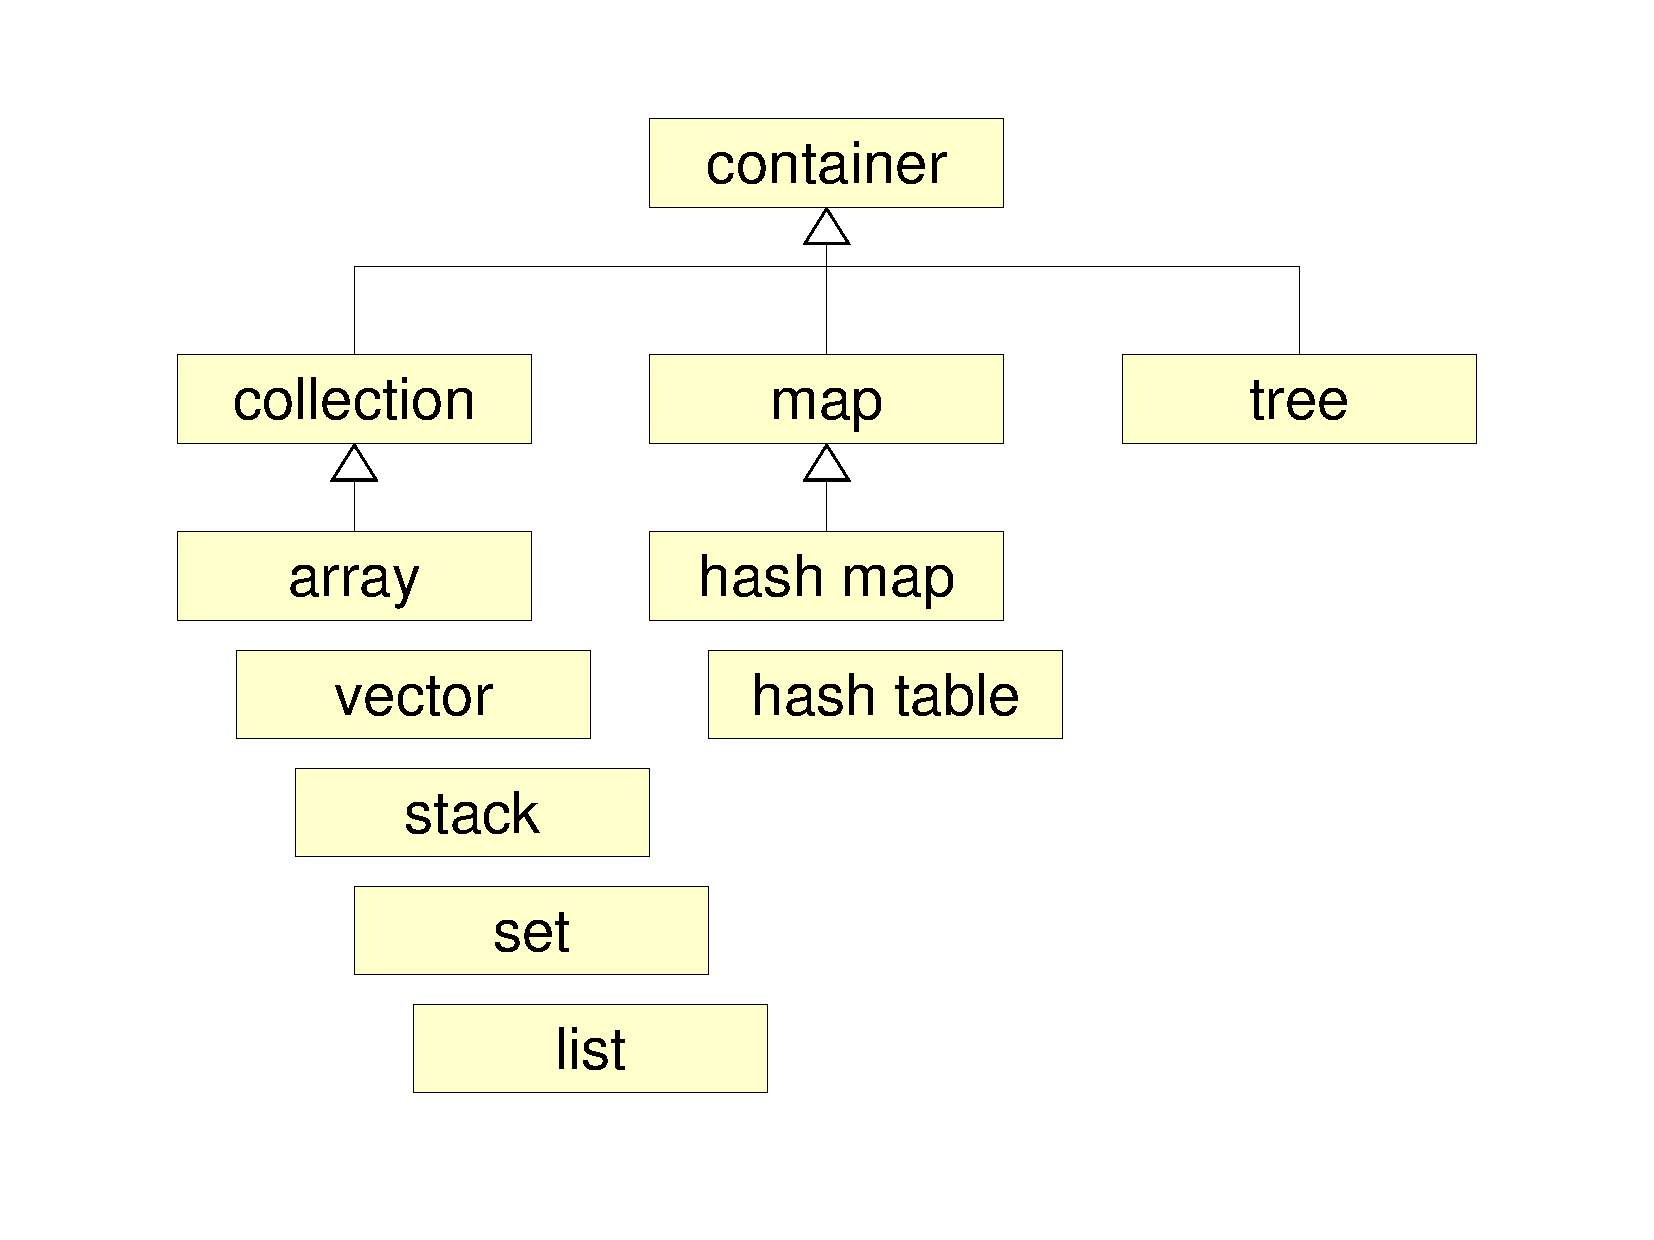
\includegraphics[scale=0.3,angle=-90]{graphics/container.pdf}
        \caption{Classical Container Types in Java}
        \label{container_figure}
    \end{center}
\end{figure}

\begin{table}[ht]
    \begin{center}
        \begin{footnotesize}
        \begin{tabular}{| p{35mm} | p{70mm} |}
            \hline
            \textbf{Classical Container Type} & \textbf{Realisation in CYBOL Knowledge Template}\\
            \hline
            Tree & Hierarchical \emph{whole}-\emph{part} structure\\
            \hline
            Table & Like a Tree, as hierarchy consisting of rows which consist of columns\\
            \hline
            Map & Parts have a \emph{name} (key) and a \emph{model} (value)\\
            \hline
            List & Parts may have a \emph{position} property\\
            \hline
            Vector & A \emph{model} attribute may hold comma-separated values;
                an extra template holds a dynamically changeable number of parts\\
            \hline
            Array & Like a Vector; characters are interpreted as \emph{string}\\
            \hline
        \end{tabular}
        \end{footnotesize}
        \caption{Mapping Classical Containers to CYBOL}
        \label{mapping_table}
    \end{center}
\end{table}

CYBOI owns a \emph{Knowledge Schema} which represents each item as
\emph{Hierarchy} by default, the result being that different types of
containers are \emph{not} needed any longer, that is are unified. Table
\ref{mapping_table} shows how the different kinds of container behaviour are
implemented in CYBOL. As can be seen, CYBOL is able to represent many container
types.
